\section{Introduction}

We consider the problem of recognizing whether a string belongs to a given language before doing the semantic analysis.
Automata are abstract machines used to describe a string recognition procedure. 

For this problem, the input domain is a set of strings of alphabet $\Sigma$. 
The application of a recognition algorithm $\alpha$ to a given string $x$ is denoted as $\alpha(x)$.
We say string $x$ is accepted if $\alpha(x)=\textnormal{yes}$, otherwise it is rejected.
The language recognized, $L(\alpha)$, is the set of accepted strings:
\[L(\alpha)=\{x \in \Sigma^{*}|\alpha(x)=\textnormal{yes}\}\]
If the language is semidecidable, it may happen that for some incorrect string $x$ the algorithm will not terminate. 
In practice, we do not have to worry about such decidability issues because in language processing the only language families of concern are decidable. 

In the theory and practice of formal languages, one computation step is a single atomic operation of the abstract recognition machine (automaton), which can manipulate only one symbol at a time.
Therefore, it is customary to present the recognition algorithm by means of an automaton of some kind, no matter if a recognizer or a transducer machine, mainly for the following reasons: 
\begin{enumerate}
    \item Outlining the correspondence between the various families of languages and the respective generative devices. 
    \item Skipping any unnecessary and premature reference to the effective implementation of the algorithm in some programming language.
\end{enumerate}
\begin{figure}[H]
    \centering
    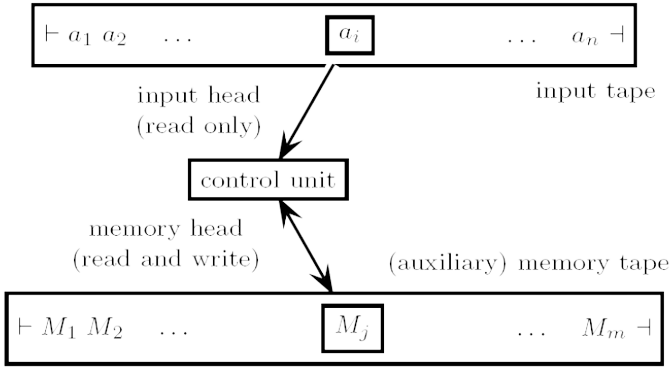
\includegraphics[width=0.3\linewidth]{images/fsa.png}
    \caption{General model of a recognizer automaton}
\end{figure}
The automata analyzes the input string and executes a series of moves. 
Each move depends on the symbols currently pointed by the heads and also on the current state. 
The move may have the following effects: 
\begin{itemize}
    \item Shifting the input head of one position to the left or right.
    \item Replacing the current memory symbol by a new one and shifting the memory head of one position to the left or right. 
    \item Changing the current state. 
\end{itemize}
Depending on the type of automata it is possible to have: 
\begin{itemize}
    \item One-way automaton: the input head can be shifted only to the right.
    \item No auxiliary memory: this is the finite state automata. 
        It is the machine model that recognizes the regular languages. 
    \item Auxiliary memory: this is the pushdown automata. 
        It is the machine model that recognizes the free languages. 
\end{itemize}
\begin{definition}
    A \emph{configuration}  is the set of the three components that determine the behavior of the automaton: 
    \begin{itemize}
        \item The still unread part of the input tape. 
        \item The contents and position of the memory tape and head, respectively. 
        \item The current state of the control unit.
    \end{itemize}
\end{definition}
In the initial configuration, the input head is positioned on the symbol immediately following the start-marker, the control unit is in a specific state (initial state), and the memory tape only contains a special initial symbol. 
The automaton configuration changes through a series of transitions, each of which is driven by a move. 
The whole series of transitions is the computation of the automaton.
\begin{definition}
    An automaton has a \emph{deterministic} behavior if in every instantaneous configuration, at most one move is possible. 
    Otherwise, the automaton is said to be \emph{non-deterministic}.
\end{definition}
In the final configuration, the control unit is in a special state qualified as final and the input head is positioned on the end-marker of the string to be recognized.
Sometimes the final configuration is characterized by a condition for the memory tape: to be empty or to contain only one special final symbol.






